\documentclass[CJK,10pt]{beamer}
%\usepackage[utf8]{inputenc}
\usepackage{xeCJK}
\usepackage{graphicx}
\usepackage{subcaption}
\usepackage {mathtools}
%\usepackage{utopia} %font utopia imported
\usetheme{CambridgeUS}
\usecolortheme{dolphin}

\usepackage{graphicx}
\usepackage{float}

% set colors
\definecolor{myNewColorA}{RGB}{25,25,112}
\definecolor{myNewColorB}{RGB}{25,25,112}
\definecolor{myNewColorC}{RGB}{25,25,112}
\setbeamercolor*{palette primary}{bg=myNewColorC}
\setbeamercolor*{palette secondary}{bg=myNewColorB, fg = white}
\setbeamercolor*{palette tertiary}{bg=myNewColorA, fg = white}
\setbeamercolor*{titlelike}{fg=myNewColorA}
\setbeamercolor*{title}{bg=myNewColorA, fg = white}
\setbeamercolor*{item}{fg=myNewColorA}
\setbeamercolor*{caption name}{fg=myNewColorA}
\usefonttheme{professionalfonts}
\usepackage{natbib}
\usepackage{hyperref}
%------------------------------------------------------------
%\titlegraphic{\includegraphics[height=1.5cm]{logo.png}} 

\setbeamerfont{title}{size=\large}
\setbeamerfont{subtitle}{size=\small}
\setbeamerfont{author}{size=\small}
\setbeamerfont{date}{size=\small}
\setbeamerfont{institute}{size=\small}



%设置页码脚标
%\setbeamertemplate{footline}[frame number]
\defbeamertemplate{footline}{NGEGFootlineTemplate}{%
	\leavevmode% 离开vmode,也就是离开竖直模式,进入水平模式
	\hbox{%
		\begin{beamercolorbox}[wd=.2\paperwidth,ht=2.25ex,dp=1ex,center]{author in head/foot}%
			\ifnum \the\value{page}>1 \usebeamerfont{author in head/foot}\insertshortauthor\fi
		\end{beamercolorbox}%
		\begin{beamercolorbox}[wd=.6\paperwidth,ht=2.25ex,dp=1ex,center]{title in head/foot}%
			\ifnum \the\value{page}>1 \usebeamerfont{title in head/foot}\insertshorttitle\fi
		\end{beamercolorbox}%
		\begin{beamercolorbox}[wd=0.2\paperwidth,ht=2.25ex,dp=1ex,center]{author in head/foot}%
			\ifnum \the\value{page}>1 \insertframenumber{} / \inserttotalframenumber\fi
	\end{beamercolorbox}}%
%	\vskip0pt%
}
\setbeamertemplate{footline}[NGEGFootlineTemplate]



\newcommand{\mb}[1]{\mathbf{#1}}
\newcommand{\mc}[1]{\mathcal{#1}}
\newcommand{\E}{\mathcal{E}}
\newcommand{\C}{\mathcal{C}}
\newcommand{\x}{\mathbf{x}}
\newcommand{\dd}{\mathrm{d}}

\newcommand{\sumFromTo}[3]{\ensuremath{\sum_{#1}^{#2} #3}}

\newcommand{\optimalProblem}[3]
{\begin{align*}
    #1 \quad &#2 \\
    \mathrm{s. t.}\quad&#3
\end{align*}}




\title[Weapon Target Assignment problem]{Weapon Target Assignment problem}%主标题
%\subtitle{ }%%副标题
\author[Guanda Li]{Guanda Li
}%%作者

\institute[LSEC]{Institute of Computational Mathematics and Scientific/Engineering Computing,\\
Academy of Mathematics and Systems Science,\\
Chinese Academy of Sciences}
\date[\textcolor{white} ]
{December 20, 2022}

%------------------------------------------------------------
%This block of commands puts the table of contents at the 
%beginning of each section and highlights the current section:
%\AtBeginSection[]
%{
%  \begin{frame}
%    \frametitle{Contents}
%    \tableofcontents[currentsection]
%  \end{frame}
%}
\AtBeginSection[]{
  \begin{frame}
  \vfill
  \centering
  \begin{beamercolorbox}[sep=8pt,center,shadow=true,rounded=true]{title}
    \usebeamerfont{title}\insertsectionhead\par%
  \end{beamercolorbox}
  \vfill
  \end{frame}
}
%------------------------------------------------------------
\AtBeginSubsection[]{
    \begin{frame}
    \vfill
    \centering
    \begin{beamercolorbox}[sep=8pt,center,shadow=true,rounded=true]{title}
        \usebeamerfont{title}\insertsubsectionhead\par%
    \end{beamercolorbox}
    \vfill
    \end{frame}
}

\begin{document}

%The next statement creates the title page.
\frame{\titlepage}
\begin{frame}
\frametitle{Contents}
\tableofcontents
\end{frame}


\section{Introduction}
\begin{frame}
    \frametitle{Background}
        \begin{itemize}
            \item Weapon Target Assignment problem is a problem in the military field
            \item The basic problem is to consider using m weapons to attack n targets, in order to minimize the weighted survival probability of all targets.
            \item The problem is proved to be {NP}-complete
        \end{itemize}
\end{frame}

\begin{frame}
    \frametitle{Basic formulation}
        
            \begin{itemize}
                \item $I = \left\{1,\cdots,m\right\} $, weapon set.
                \item $J = \left\{1,\cdots,n\right\} $, target set.
                \item $p_{ij}\in [0,1]$, probability that $i$ hits $j$
                \item $V_j$, weight of the target $j$.
                \item $x_{ij}$, decision variables, whether weapon $i$ attack $j$.
            \end{itemize}
    
    \begin{align*} \tag{S0}
        \max\quad & \sum_{j=1}^n V_j \left( 1 - \prod_{i=1}^m (1 -  p_{ij})^{x_{ij}} \right) \\ 
        \mathrm{s. t.}\quad &\sum_{j=1}^n x_{ij} \leq 1\quad \forall ~i \in I,\\
        & x_{ij} \in \left\{ 0,1 \right\} \quad \forall~ j\in J , ~ i \in I.
    \end{align*}
\end{frame}


\begin{frame}
    \frametitle{Basic formulation}
     \begin{itemize}
    	\item $I = \left\{1,\cdots,m\right\} $, weapon set.
    	\item $J = \left\{1,\cdots,n\right\} $, target set.
    	\item $p_{ij}\in [0,1]$, probability that $i$ hits $j$
    	\item $V_j$, weight of the target $j$.
    	\item $x_{ij}$, decision variables, whether weapon $i$ attack $j$.
    \end{itemize}
    
    \begin{align*} \tag{S0'}
        \min\quad & \sum_{j=1}^n V_j \left( \prod_{i=1}^m (1 -  p_{ij})^{x_{ij}} \right) \\ 
        \mathrm{s. t.}\quad &\sum_{j=1}^n x_{ij} \leq 1\quad \forall ~i \in I,\\
        & x_{ij} \in \left\{ 0,1 \right\} \quad \forall~ j\in J , ~ i \in I.
    \end{align*}
\end{frame}

\begin{frame}
    \frametitle{Weapon target assignment problem}
    \begin{figure}[H]
        \centering
        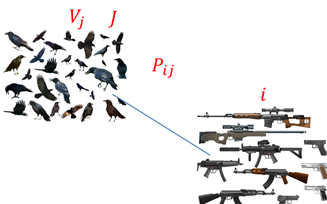
\includegraphics[width=0.7\textwidth]{20221220150429.png}
        \caption{WTA problem} 
        \label{Fig.main2} 
        \end{figure}
\end{frame}

\begin{frame}
    \frametitle{History}
    \begin{itemize}
        \item Manne (1958)\\
         Give the basic formulation of the problem. Solve the problem with linear approximations to problems, exactly solve small-scale problems.
         \item denBroeder (1959) , Hosein(1989) \\
         solve a simpler model assume that all the weapon has the same probability of hitting the same target.
         \item Lloyd Witsenhause (1986) \\ Prove the problem is NP-complete.
         \item Johansson Falkman (2009) \\ Use search algorithm solve the problem with 9 weapons and 8 targets in 13 minutes.
         \item Rosenberger et al. (2005), Ahuja et al. (2007), Kline (2017)
         \\Use branch-and-bound frame work to solve the WTA problem. It takes 16.2 hours to solve the model with size 80 weapons and 80 targets. 
    \end{itemize}
\end{frame}



\begin{frame}
    \frametitle{History}
    \begin{itemize}
        \item Lu(2021)\\ Transform the problem into a huge size linear programming and use column enumeration to solve the problem.
        \item Anderson(2022)\\ Use lower linear approximation of the objective function in a branch-and-bound framework.
        \item These two new techniques significantly improved the computation efficiency. Both of them could solve the problem with size 400 weapons and 400 targets in a few minutes.
    \end{itemize}
\end{frame}



\section{Formulations and Algorithms}

%\begin{frame}
%    \frametitle{Category}
%    \begin{itemize}
%        \item Static WTA problems.
%        \item Dynamic WTA problems
%        \item New developments.
%        \item My work is focus on Static WTA problems.
%    \end{itemize}
%\end{frame}


%\begin{frame}
%    \frametitle{Notation}
%    \begin{columns}
%        \begin{column}{.50\linewidth}
%            \footnotesize
%            \begin{itemize}
%                \item $I$, weapon set.
%                \item $J$, target set.
%                \item $n$, number of targets.
%                \item $m$, number of weapon types. If limiting to one of each type, this variable indicates the number of weapons.
%                \item $w_i$, the number of class i weapon
%            \end{itemize}
%        \end{column}
%        \begin{column}{.50\linewidth}
%            \footnotesize
%            \begin{itemize}
%                \item $p_{ij}$, probability that weapon i hits target j.
%                \item $q_{ij}$, probability that weapon i misses target j.
%                \item $x_{ij}$, number of weapons of type i assigned to target j. If each weapon is limited to only one, this variable is a 0-1 variable.
%                \item $V_j$, value of target j.
%                \item $c_{ij}$, cost of assigning weapon i to target j
%            \end{itemize}
%        \end{column}
%    \end{columns}
%\end{frame}

\begin{frame}
    \frametitle{WTA model 1}
    \begin{itemize}
        \item Compared to the basic model, allows $w_i$ weapons for each weapon type.
    \end{itemize}
    \begin{align*} \tag{S1}
        \min\quad & \sum_{j=1}^n V_j \left( \prod_{i=1}^m (1 -  p_{ij})^{x_{ij}} \right) \\ 
        \mathrm{s. t.}\quad &\sum_{j=1}^n x_{ij} \leq w_i\quad \forall ~i \in I,\\
        & x_{ij} \in \mathbb{Z}^+ \quad \forall~ j\in J , ~ i \in I.
    \end{align*}
    
\end{frame}
%\begin{frame}
%    \frametitle{WTA model 1}
%    \begin{itemize}
%        \item Transform $1-p_{ij}$ to $q_{ij}$ to make the formulation simpler.
%    \end{itemize}
%    \begin{align*} \tag{S1.2}
%        \min\quad & \sum_{j=1}^n V_j \left( \prod_{i=1}^m q_j^{x_{ij}} \right) \\ 
%        \mathrm{s. t.}\quad &\sum_{j=1}^n x_{ij} \leq w_i\quad \forall ~i \in I,\\
%        & x_{ij} \in \mathbb{Z}^+ \quad \forall~ j\in J , ~ i \in I.
%    \end{align*}
%\end{frame}

\begin{frame}
    \frametitle{WTA model 2}
    \begin{itemize}
        \item For convenience, assume that any weapon has the same probability of  hitting the same target.
    \end{itemize}
    \begin{align*} \tag{S2}
        \min\quad & \sum_{j=1}^n V_j (1-p_{j})^{\sum_{i=1}^m x_{ij}} \\ 
        \mathrm{s. t.}\quad &\sum_{j=1}^n x_{ij} \leq w_i\quad \forall ~i \in I,\\
        & x_{ij} \in \mathbb{Z}^+ \quad \forall~ j\in J , ~ i \in I.
    \end{align*}
\end{frame}

\begin{frame}
    \frametitle{WTA model 3}
    \begin{itemize}
        \item Logarithm of the objective function in S1
    \end{itemize}
    \begin{align*} \tag{S3.1}
        \min\quad & \sum_{j=1}^n V_j \exp \left( \sum_{i=1}^m {x_{ij}\ln(1 -  p_{ij})} \right) \\ 
        \mathrm{s. t.}\quad &\sum_{j=1}^n x_{ij} \leq w_i\quad \forall ~i \in I,\\
        & x_{ij} \in \mathbb{Z}^+ \quad \forall~ j\in J , ~ i \in I.
    \end{align*}
\end{frame}

\begin{frame}
    \frametitle{WTA model 3}
    \begin{itemize}
        \item Replaced the objective function with $y_j$ to get the following model.
    \end{itemize}
    \begin{align*} \tag{S3.2}
        \min\quad & \sum_{j=1}^n V_j e^{y_j}  \\ 
        \mathrm{s. t.}\quad &\sum_{j=1}^n x_{ij} \leq w_i\quad \forall ~i \in I,\\
        & \sum_{i=1}^m {\ln(1 -  p_{ij}) x_{ij}} = y_j \quad \forall ~ j \in J\\
        & x_{ij} \in \mathbb{Z}^+ \quad \forall~ j\in J , ~ i \in I.
    \end{align*}
    \begin{itemize}
        \item The model is equivalent to model S1, but it is more convenient for the solver to calculate.
        \item \textcolor{blue}{Kline et al.(2017b)} points out that use the commercial solver BARON to solve the problem, this form can increase the correct rate by 21\%
    \end{itemize}
\end{frame}



\begin{frame}
    \frametitle{WTA model 4}
    \begin{itemize}
        \item Limit the $x_{ij}$ to bianry variable.
        \item For $(1-p_{ij}x_{ij}) = (1-p_{ij})^{x_{ij}},~ x \in \left\{ 0,1\right\}$,The problem can be transformed into the following form.
    \end{itemize}
    \begin{align*} \tag{S4}
        \min\quad & \sum_{j=1}^n V_j \left( \prod_{i=1}^m (1 -  p_{ij}x_{ij}) \right) \\ 
        \mathrm{s. t.}\quad &\sum_{j=1}^n x_{ij} \leq 1\quad \forall ~i \in I,\\
        & x_{ij} \in \left\{ 0,1 \right\} \quad \forall~ j\in J , ~ i \in I.
    \end{align*}
    \begin{itemize}
        \item This conversion will cause the relaxation of the problem from a convex from to a non-convex form.
    \end{itemize}
\end{frame}

\begin{frame}
    \frametitle{WTA model 5}
    \begin{itemize}
        \item Transform the problem into a knapsack problem
    \end{itemize}
    \begin{align*} \tag{S5}
        \min\quad & \sum_{j=1}^n{\sum_{x=1}^m{c_{ij}x_{ij}}} \\ 
        \mathrm{s. t.}\quad &\sum_{j=1}^n x_{ij} \leq 1\quad \forall ~i \in I,\\
        & \sum_{i=1}^m x_{ij} \leq 1\quad \forall ~j \in J \\
        & x_{ij} \in \left\{ 0,1 \right\} \quad \forall~ j\in J , ~ i \in I.
    \end{align*}
    \begin{itemize}
        \item This method removes the coupling when multiple weapons strike the same weapon, transforms the difficult objective function into a linear function.
    \end{itemize}
\end{frame}


\section{Outer Approximation}


\begin{frame}
	\frametitle{Basic formulation}
	\begin{itemize}
		\item $I = \left\{1,\cdots,m\right\} $, weapon set.
		\item $J = \left\{1,\cdots,n\right\} $, target set.
		\item $p_{ij}\in [0,1]$, probability that $i$ hits $j$
		\item $V_j$, weight of the target $j$.
		\item $x_{ij}$, decision variables, whether weapon $i$ attack $j$.
	\end{itemize}
	
	\begin{align}
		\min\quad & \sum_{j=1}^n V_j \left( \prod_{i=1}^m (1 -  p_{ij})^{x_{ij}} \right) \\ 
		\mathrm{s. t.}\quad &\sum_{j=1}^n x_{ij} \leq 1\quad \forall ~i \in I,\\
		& x_{ij} \in \left\{ 0,1 \right\} \quad \forall~ j\in J , ~ i \in I.
	\end{align}
\end{frame}


\begin{frame}
    \frametitle{Convexity of the objective function}
    \begin{equation*}
        f_j(x) =  \prod_{i=1}^m (1 -  p_{ij})^{x_{ij}}\quad \forall~  j \in J
    \end{equation*}
    Hessian matrix $H$:
    \begin{equation*}
        \frac{\partial f_j(x)}{\partial x_{aj} \partial x_{bj}} = \ln(1 - p_{aj}) \ln(1 - p_{bj}) f_j(x)
    \end{equation*}
    {
    \scriptsize
    \begin{equation*}
        H = f(x)\begin{bmatrix}
            \ln(1 - p_{1j}) \ln(1 - p_{1j}) & \ln(1 - p_{1j}) \ln(1 - p_{2j}) &\cdots & \ln(1 - p_{1j}) \ln(1 - p_{mj}) \\
            \ln(1 - p_{2j}) \ln(1 - p_{1j}) & \ln(1 - p_{2j}) \ln(1 - p_{2j}) &\cdots & \ln(1 - p_{2j}) \ln(1 - p_{mj}) \\
            \vdots & \vdots &\ddots &\vdots \\
            \ln(1 - p_{mj}) \ln(1 - p_{1j}) & \ln(1 - p_{mj}) \ln(1 - p_{2j}) &\cdots & \ln(1 - p_{mj}) \ln(1 - p_{mj})
        \end{bmatrix}
    \end{equation*}
    }
\end{frame}

\begin{frame}
    \frametitle{Convexity of the objective function}
    Let
    \begin{equation*}
        l = \begin{bmatrix}
            \ln(1 - p_{1j}) & \ln(1 - p_{2j}) & \cdots & \ln(1 - p_{mj})
        \end{bmatrix}
    \end{equation*}
    Hessian matrix is :
    \begin{equation*}
        H = f(x)l\cdot l^T
    \end{equation*}
    The Hessiann matrix is a rank-one matrix so the objective function is convex.
\end{frame}

\begin{frame}
    \frametitle{Transformed model}
    Objective function
    \begin{equation*}
        \sum_{j=1}^n a_j \left( \prod_{i=1}^m (1 -  p_{ij})^{x_{ij}} \right)
    \end{equation*}
    {\footnotesize
    By introducing auxiliary variables, the nonlinear term can be transformed from the objective function into the constraint.
    
    If we take $\eta_j$ as the auxiliary variables to $\prod_{i=1}^m (1 -  p_{ij})^{x_{ij}}$ the model can be transformed to 
    \begin{align*} \tag{S0'}
        \min\quad & \sum_{j=1}^n a_j \eta_j \\ 
        \mathrm{s. t.}\quad & \eta_j \geq \prod_{i=1}^m (1 -  p_{ij})^{x_{ij}}, \quad \forall ~ j \in J \\ 
        &\sum_{j=1}^n x_{ij} \leq 1\quad \forall ~ i \in I,\\
        & x_{ij} \in \left\{ 0,1 \right\} \quad \forall ~ j\in J\quad i \in I.
    \end{align*}
    }
\end{frame}

\begin{frame}
    \frametitle{Basic idea of outer approximation}
    If $f(x)$ is a convex function, then for any point $x^*$ in the feasible region, we have
    \begin{equation*}
        f(x) \geq f(x^*) + \nabla f(x^*)(x - x^*)
    \end{equation*}
    Therefore, if the constraint of the original problem is $\eta \geq f(x)$, then
    \begin{equation*}
        \eta \geq f(x) \geq f(x^*) + \nabla f(x^*)(x - x^*)
    \end{equation*}
    must be correct
    \begin{itemize}
        \item For any given point, a linear constraint can be introduced to ensure that the feasible region satisfies the constraint.
        \item The outer approximation method try to replace a nonlinear constraint by some linear constraints, but guarantees the models are equivalent.
    \end{itemize}
    
    
\end{frame}

\begin{frame}
    \frametitle{Outer approximation constraint}
    take $f_j(x) =  \prod_{i=1}^m (1 -  p_{ij})^{x_{ij}}\quad j \in J$,then for any given  $\bar{x}$ in feasible domain, we have 
    \begin{align*}
        \nabla f(\bar{x})(x - \bar{x}) & = f(\bar{x})\sum_{i = 1}^m \ln(1-p_{ij})(x_{ij} - \bar{x_{ij}})\\
        &= f(\bar{x})\sum_{i = 1}^m \ln(1-p_{ij})x_{ij} - f(\bar{x})\sum_{i = 1}^m \ln(1-p_{ij})\bar{x_{ij}}
    \end{align*}
    \begin{itemize}
        \item We denote this constraint as the outer approximation constraint.
    \end{itemize}
    

    
\end{frame}

\begin{frame}
    \frametitle{Outer approximation model}
    Let $X$ donates the set of all integer feasible solutions in the problem, the model can be described as.
    {\scriptsize
    \begin{align*} \tag{OA}
        \min\quad & \sum_{j=1}^n a_j \eta_j \\ 
        \mathrm{s. t.}\quad & \eta_j \geq f(\bar{x})\sum_{i = 1}^m \ln(1-p_{ij})(x_{ij} - \bar{x}_{ij}) + f(\bar{x}), \quad \forall ~ j \in J,\ \bar{x} \in X \\ 
        &\sum_{i=1}^m x_{ij} \leq 1\quad \forall ~ j \in J,\\
        & x_{ij} \in \left\{ 0,1 \right\} \quad \forall ~ j\in J\quad i \in I.
    \end{align*}
    }
    the number of outer approximation constraints is very large. The restricted model only take care of some of them.
   
\end{frame}

\begin{frame}
    \frametitle{Idea of outer approximation method}
    We assume that $\hat{X} \subseteq X$.
    {
    \scriptsize
    
    \begin{align*}
        \min\quad & \sum_{j=1}^n a_j \eta_j \\ 
        \mathrm{s. t.}\quad & \eta_j \geq f(\bar{x})\sum_{i = 1}^m \ln(1-p_{ij})(x_{ij} - \bar{x_{ij}}) + f(\bar{x}), \quad j \in J,\ \bar{x} \in \hat{X} \\ 
        &\sum_{i=1}^m x_{ij} \leq 1\quad j \in J,\quad x_{ij} \in \left\{ 0,1 \right\} \quad j\in J\quad i \in I
    \end{align*}
    }
\end{frame}

\begin{frame}
    \frametitle{Algorithm of outer approximation}
    \begin{enumerate}
        \item Remove all outer approximation constraints and give the current optimal solution $x, \eta$
        \item Check whether the current optimal solution can satisfy all the outer approximation constraints. if true, the iteration terminates and end the execution.
        \item Otherwise, choose to outer approximation constraint that has been violate most and add it to the restricted model, resolve the model and go to step 2.
    \end{enumerate}
\end{frame}


\begin{frame}
    \frametitle{Choose violated constraint}
    {
    \scriptsize
    \begin{align*}
        \min\quad & \sum_{j=1}^n a_j \eta_j \\ 
        \mathrm{s. t.}\quad & \eta_j \geq f(\bar{x})\sum_{i = 1}^m \ln(1-p_{ij})(x_{ij} - \bar{x}_{ij}) + f(\bar{x}), \quad j \in J,\ \bar{x} \in X \\ 
        &\sum_{i=1}^m x_{ij} \leq 1\quad j \in J,\quad x_{ij} \in \left\{ 0,1 \right\} \quad j\in J\quad i \in I
    \end{align*}
    }
    \begin{itemize}
        \item Unless an optimal solution has been found, the solution to the restricted problem must bring a violation of the outer approximation constraint.
        \item When obtaining a solution that $x$ is in the feasible region, if $\eta < f_j(x)$, this causes infeasible. the infeasible point can be excluded by adding an outer approximation constraint.
    \end{itemize}
\end{frame}

\begin{frame}
    \frametitle{Numerical results}
    Weapon-Target Assignment Problem Instances \footnote{Emrullah SONUC, Baha SEN, and Safak BAYIR, A Parallel Simulated Annealing Algorithm for 
     Weapon-Target Assignment Problem, International Journal of Advanced Computer Science and Applications,
     8(4), 2017}
    \begin{itemize}
     \item SET1: Only to separate integer infeasible solutions.
     \item SET2: Also to separate fractional infeasible solutions.
    \end{itemize}
    \begin{table}
     \begin{tabular}{|c|c|c|c|c|}\hline
       & \multicolumn{2}{|c|}{SET1}& \multicolumn{2}{|c|}{SET2} \\\hline
      $|I|\times |J|$ &  time(s) & nodes &  time(s) & nodes\\\hline
      $5\times 5$ & 0.20 & 2 &  0.20 & 2\\\hline
      $10\times 10$ &  0.01 & 9 &  0.01 & 3\\\hline
      $20\times 20$ & 0.38 & 1680 &  0.28 & 69\\\hline
      $30\times 30$ & 152.49 & 491403 &  40.40 & 16932\\\hline
      $40\times 40$ & 3600.00+ & -- &  77.14  & 38967 \\\hline
      $50\times 50$ & 3600.00+ & -- & 3600.00+ & -- \\\hline 
     \end{tabular}
    \end{table}
   \end{frame}


\section{Columnn Generation}
\begin{frame}
    \frametitle{Basic Idea}
    \begin{itemize}
        \item Some linear programming problems have too many columns (variables), making it difficult to solve
        \item Use only some of the variables at the beginning of the algorithm and assume all the other variables are 0
        \item Variables that have the potential to improve the objective function are iteratively added to the model. 
        \item Once it can be proven that adding new variables will no longer improve the value of the objective function, the iterative process is terminated and an optimal solution is obtained.
    \end{itemize}
\end{frame}

\begin{frame}
    \frametitle{How to use column generation in WTA Problem}
    \begin{itemize}
		\item \textbf{Basic Idea}:By listing all the weapon assignment scenarios $S$, the problem is transformed into a linear programming problem.
		\item Assuming that there are $m$ weapons, for any target $j$, each weapon can choose to attack $j$ or not attack $j$, so there are $2^m$ different attack schemes.
		\item \textbf{an example}:There are a total of 8 weapons, and the attack plan using No. 1, 3, and 6 weapons is recorded as $s_{[1,0,1,0,0,1,0,0]}$, $|S| = 2^8 = 256$
		\item $n_{si}$: bianry variable, indicates whether to enable weapon $i$ in the $s$th scene. In the above example, $n_{s1} = 1,\ n_{s2} = 0$
		\item $q_{js} = a_j \prod_{i = 1}^m (1 - n_{si}\cdot p_{ij})$:weighted probability of the plan $s$ to hit the target $j$,For example, $q_{3s}$ is to use the No. 1, 3, and 6 weapons to hit the target $3$ and multiply the probability of destroying the target $j$ by the weight of the target $j$.
	\end{itemize}
\end{frame}

\begin{frame}
    \frametitle{Transformed formulation}
    \optimalProblem{\min}{\sumFromTo{j = 1}{n}{\sumFromTo{s = 0}{2^m -1}{q_{js}y_{js}}}\tag{CG}}{\sumFromTo{j = 1}{n}{\sumFromTo{s = 0}{2^m -1}{n_{si}y_{js}}}\leq 1 \quad &\forall ~ i \in I\\& \sumFromTo{s = 0}{2^m - 1}{y_{js}} = 1 \quad &\forall ~ j \in J\\& y_{js} \in \left\{ 0,1 \right\} &\forall ~ j\in J,\ s\in S}
    \begin{columns}
        \begin{column}{.55\linewidth}
            \footnotesize
            \begin{itemize}
                \item $I = \left\{1,\cdots,m\right\} $, weapon set
                \item $J = \left\{1,\cdots,n\right\} $, target set
                \item $S = \left\{1,\cdots,2^m\right\}$, scene set
            \end{itemize}
        \end{column}
    \hspace{-3cm}
        \begin{column}{.55\linewidth}
            \footnotesize
            \begin{itemize}
                \item $n_{si}$:weather scene $s$ use weapon $i$
                \item $y_{js}$:Whether use $s$ to arrack target $j$
                \item $q_{js}$:weighted destruction probability of using $s$ to $j$
            \end{itemize}
        \end{column}
    \end{columns}
\end{frame}

\begin{frame}
    \frametitle{Transformed formulation continuous}
    \optimalProblem{\min}{\sumFromTo{j = 1}{n}{\sumFromTo{s = 0}{2^m -1}{q_{js}y_{js}}}\tag{CG}}{\sumFromTo{j = 1}{n}{\sumFromTo{s = 0}{2^m -1}{n_{si}y_{js}}}\leq 1 \quad &\forall ~ i \in I\\& \sumFromTo{s = 0}{2^m - 1}{y_{js}} = 1 \quad &\forall ~ j \in J\\& y_{js} \in \left\{ 0,1 \right\} & \forall ~ j\in J,\ s\in S}
    \begin{itemize}
        \item \textbf{objective function}:minimize the weighted destruction probabilities.
        \item \textbf{first constraint}:each weapon can only attack one target.
        \item \textbf{second constraint}:assign exactly one scene for each target
    \end{itemize}
\end{frame}

\begin{frame}
    \frametitle{Column enumeration}
    \optimalProblem{\min}{\sumFromTo{j = 1}{n}{\sumFromTo{s = 0}{2^m -1}{q_{js}y_{js}}}\tag{CG}}{\sumFromTo{j = 1}{n}{\sumFromTo{s = 0}{2^m -1}{n_{si}y_{js}}}\leq 1 \quad &\forall ~ i \in I\\& \sumFromTo{s = 0}{2^m - 1}{y_{js}} = 1 \quad &\forall ~ j \in J\\& y_{js} \in \left\{ 0,1 \right\} & \forall ~ j\in J,\ s\in S}

    \begin{itemize}
        \item This idea is from \textcolor{blue}{Lu(2021)}
        \item The basic idea of the column enumeration method is to enumerate all columns in a smarter way
        \item Two techniques are used in the article: weapon number bounding and weapon domination
        \item weapon number bounding:Scenarios with too few or too many weapons are give no improvement to the objective function.
        \item weapon domination:For a certain target, it is better to arrange one weapon than another
    \end{itemize}
\end{frame}




\begin{frame}
    \frametitle{LP Relaxition}
    \optimalProblem{\min}{\sumFromTo{j = 1}{n}{\sumFromTo{s = 0}{2^m -1}{q_{js}y_{js}}}\tag{CG-LP}}{\sumFromTo{j = 1}{n}{\sumFromTo{s = 0}{2^m -1}{n_{si}y_{js}}}\leq 1 \quad &\forall ~ i \in I\\& \sumFromTo{s = 0}{2^m - 1}{y_{js}} = 1 \quad &\forall ~  j \in J\\& y_{js} \geq 0 &\forall ~ j\in J,\ s\in S}
    \begin{itemize}
        \item LP Relaxition, the third constraint can be changed into $y_{js} \geq 0$
        \item Linear program contains $n \times 2^m$ columns
        \item Only some of the columns (variables) are taken, because in the optimal solution of linear programming, at most $m+n$ variables are not 0, that is, the dual constraints corresponding to other variables are not active.
    \end{itemize}
\end{frame}

\begin{frame}
    \frametitle{Dual Problem}
    
    \optimalProblem{\max}{\sumFromTo{i=1}{m}{u_i} + \sumFromTo{j=1}{n}{v_j}\tag{CG-Dual}}{\sumFromTo{i=1}{m}{x_{is}u_i}+ v_j \leq q_{js}\quad \forall ~(s,j) \in X\\ &u_i \leq 0,\quad v_j\ \mathrm{free}}
    \begin{itemize}
        \item If $X = \left\{(s,j) | s\in S , j \in J \right\}$, each element in $X$ corresponds to a constraint.
        \item \item Selecting some columns in the original problem is equivalent to selecting some rows in the dual problem.
    \end{itemize}
\end{frame}

\begin{frame}
    \frametitle{Restricted Dual Problem}
    
    \optimalProblem{\max}{\sumFromTo{i=1}{m}{u_i} + \sumFromTo{j=1}{n}{v_j}\tag{CG-Dual-R}}{\sumFromTo{i=1}{m}{x_{is}u_i}+ v_j \leq q_{js}\quad ~\forall (s,j) \in \hat{X} \\ &u_i \leq 0,\quad v_j\ \mathrm{free}}
    \begin{itemize}
        
        \item Only select some constraints, that is, only consider the constraints generated by the some $(s,j)$ in $\hat{X} \subseteq X$
        \item Solve to get $u^*, v^*$ and bring into the original dual, if all the constraints are satisfied, it must be the optimal solution.
        \item Otherwise, choose the constraint that violates the most, that is, the largest $\sumFromTo{i=1}{m}{x_{is}u_i}+ v_j > q_{js}$.
    \end{itemize}
\end{frame}

\begin{frame}
    \frametitle{Subproblem}
    \optimalProblem{\min}{a_j \prod_{i=1}^{m}{(1-p_{ij}x_{is})} -\sumFromTo{i=1}{m}{x_{is}}u_i - v_j}{j \in J,\quad s \in S\tag{CG-sub}}
    \begin{itemize}
        \item Choose the constraint that violates the most, that is, the largest $\sumFromTo{i=1}{m}{x_{is}u_i}+ v_j > q_{js}$.
        \item Using the definition of $q_{js}$ to get the above sub-problems.
        \item The problem can be separated and then solved for each given target $j$.
        \item It is intuitive that using each weapon to attack requires a cost, we try  to balance the cost of the weapon and the probability of destroying the target.
    \end{itemize}
\end{frame}

\begin{frame}
    \frametitle{Motivation to use column generation}
    \begin{itemize}
        \item Huge improvement in computational result for column enumerations
        \item The article on column enumeration mentions that column generation subproblems is hard to solve due to non-linearity
        \item The outer approximation method can be used in subproblems
    \end{itemize}
\end{frame}

\section{Future Work}
\begin{frame}
    \frametitle{Use column generation in $S1$}
    \begin{align*} \tag{S1}
        \min\quad & \sum_{j=1}^n V_j \left( \prod_{i=1}^m (1 -  p_{ij})^{x_{ij}} \right) \\ 
        \mathrm{s. t.}\quad &\sum_{j=1}^n x_{ij} \leq w_i\quad \forall ~i \in I,\\
        & x_{ij} \in \mathbb{Z}^+ \quad \forall~ j\in J , ~ i \in I.
    \end{align*}
\end{frame}

\begin{frame}
    \frametitle{More comlicated model}
    \begin{itemize}
        \item Dynamic WTA problem.
        \item muti-objective WTA problem.
        \item Sensor WTA problem.
    \end{itemize}
\end{frame}

\begin{frame}
\textcolor{myNewColorA}{\Huge{\centerline{Thank you!}}}
\end{frame}


\end{document}